\documentclass{beamer}


\usepackage{amsmath}
\usepackage[style=alphabetic,url=true]{biblatex}
\usepackage{environ}
\usepackage{geometry}
\usepackage{graphicx}
\usepackage{tikz}
\usepackage[T2A]{fontenc}
\usepackage[utf8]{inputenc}
\usepackage[cache=false]{minted}
\usepackage{amsmath}
\usepackage{amsfonts}
\usepackage{amssymb}
\usepackage{calrsfs}


% \usetheme{Bergen}

\usecolortheme{beaver}

\setbeamertemplate{itemize item}[circle]
\setbeamertemplate{itemize subitem}{--}
\addtobeamertemplate{navigation symbols}{}{
  \usebeamerfont{footline}%
  \usebeamercolor[fg]{footline}%
  \hspace{1em}%
  \insertframenumber/\inserttotalframenumber
}
\graphicspath{ {./graphics/} }
\setminted[Python]{
  fontsize=\tiny
}
\BeforeBeginEnvironment{minted}{\medskip}
\AfterEndEnvironment{minted}{\medskip}



\title{
  Bitcoin and Cryptocurrency Technologies \\
  Lecture 3: Cryptography Basics 2/2
}

\author{Yuri Zhykin}
\date{Mar 2, 2023}

\begin{document}

\frame{\titlepage}

\begin{frame}
  \frametitle{Public-key Cryptography Recap}
  \begin{itemize}
  \item \textbf{Public-key cryptography} or \textbf{asymmetric cryptography}
    involves cryptographic systems that use \textbf{pairs} of keys:
    \begin{itemize}
    \item \textbf{private keys}, which must be kept secret and only known to the
      owner,
    \item \textbf{public keys}, which may be known to others.
    \end{itemize}
  \item The core idea behind public-key cryptography is that anyone who knows
    the public key, can ``lock'' some information with that key in a way that
    only the owner of the private key can ``unlock'' it.
  \item Introduced by Ralph Merkle, Whitfield Diffie, Martin Hellman and others
    in 1970s.
  \item Arguably the only reason why it's possible to do anything useful over
    the Internet.
  \end{itemize}
\end{frame}

\begin{frame}
  \frametitle{Diffie-Hellman Key Exchange Protocol 1/2}
  \begin{itemize}
  \item Diffie-Hellman-Merkle key exchange algorithm can be intuitively
    explained with the following example:
  \end{itemize}
  \begin{center}
    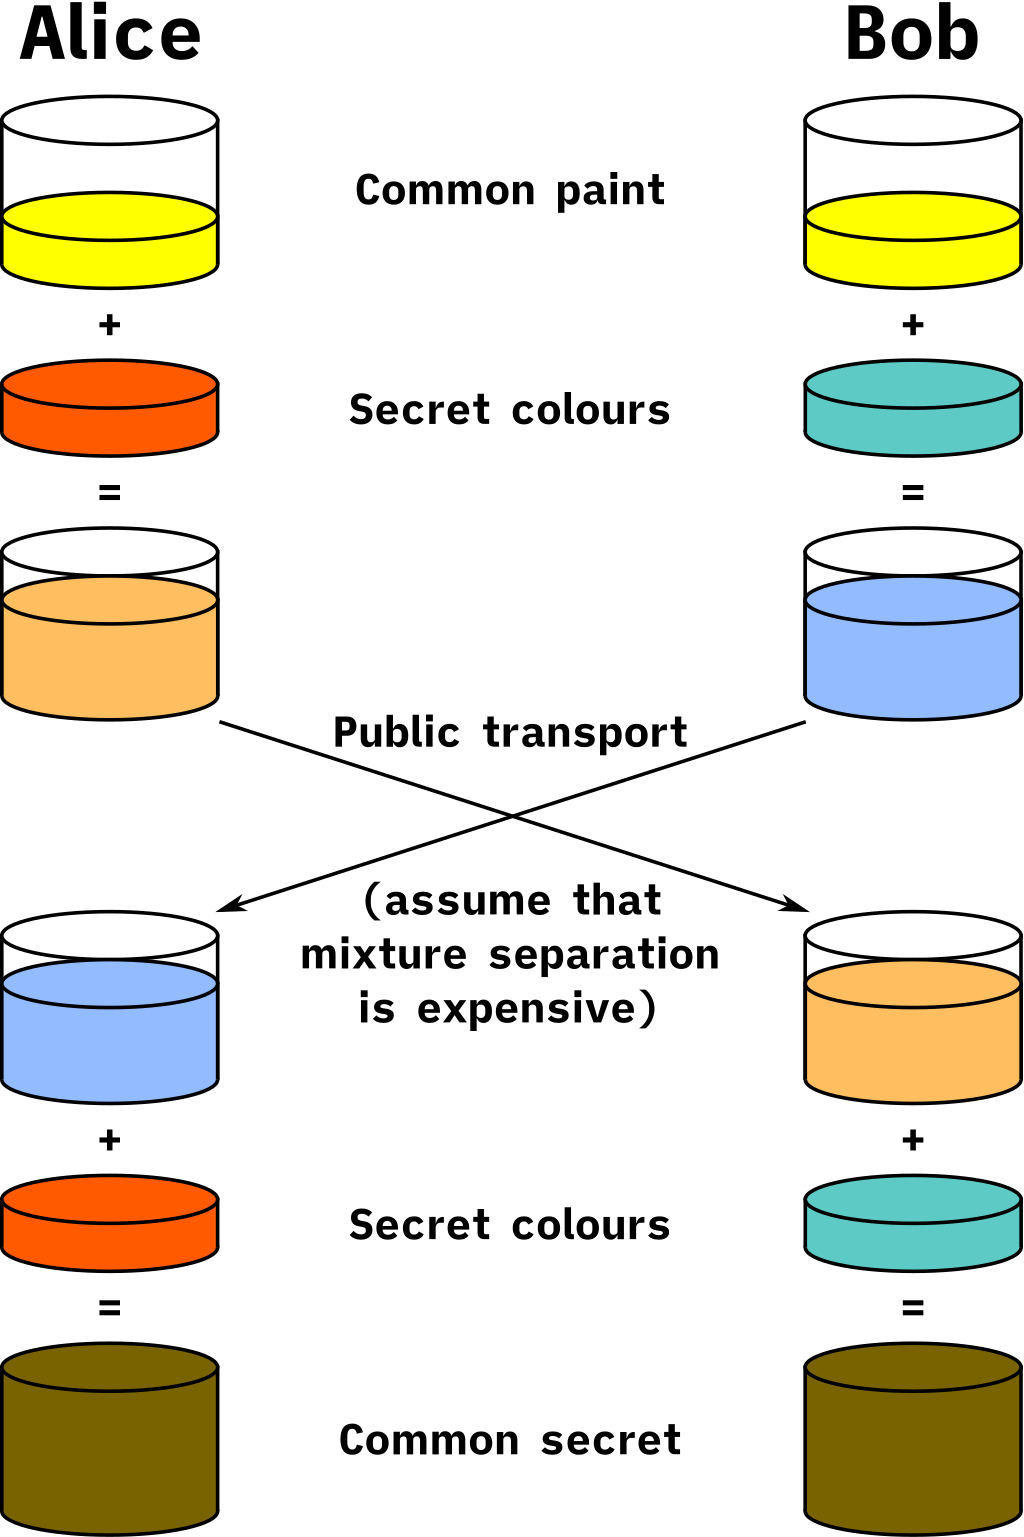
\includegraphics[width=0.35\textwidth]{dh}
  \end{center}
\end{frame}

\begin{frame}
  \frametitle{Diffie-Hellman Key Exchange Protocol 2/2}
  \begin{itemize}
  \item DH protocol implementations are based on the following observation
    written additively
    \begin{align*}
      A &= aG (= G + G + ... + G) \\
      B &= bG \\
      bA &= b(aG) = (ba)G = (ab)G = a(bG) = aB
    \end{align*}
    or multiplicatively
    \begin{align*}
      A &= G^a (= G * G * ... * G) \\
      B &= G^b \\
      A^b &= (G^a)^b = G^{(ab)} = G^{(ba)} = (G^b)^a = B^a
    \end{align*}
  \end{itemize}
\end{frame}

\begin{frame}
  \frametitle{Fields 1/2}
  \begin{itemize}
  \item A \textbf{field} is a set with defined \textbf{addition},
    \textbf{subtraction}, \textbf{multiplication} and \textbf{division}
    operations that follow the \textbf{field axioms}:
    \begin{align*}
      &\forall a, b, c: (a \star b) \star c = a \star (b \star c) \text{ -
        associativity for $+$ and $*$} \\
      &\forall a, b: a \star b = b \star a \text{ - commutativity for $+$ and
        $*$} \\
      &\exists e_+ = 0: \forall a: e + a = 0 + a = a \text{ - additive identity}
      \\
      &\exists e_* = 1: \forall a: e * a = 1 * a = a \text{ - multiplicative
        identity} \\
      &\forall a: \exists (-a): a + (-a) = e_+ = 0 \text{ - additive inverse} \\
      &\forall a \neq 0: \exists (a^{-1}): a * (a^{-1}) = e_* = 1 \text{ -
        multiplicative inverse} \\
      &\forall a, b, c: a*(b+c) = (a*b) + (a*c) \text{ - $*$ over $+$
        distributivity} \\
    \end{align*}
  \end{itemize}
\end{frame}

\begin{frame}
  \frametitle{Fields 2/2}
  \begin{itemize}
  \item Set of \textbf{rational numbers} $\mathbb{R}$ is a field over regular
    addition and multiplication.
  \item In cryptography, we usually consider \textbf{finite (Galois) fields}
    with \textbf{prime order} over modular arithmetic operations:
    $$F_n = \mathbb{Z}/n\mathbb{Z} = {0, 1, ..., n - 1}$$
    where $n$ is a prime number; note that \textbf{this construction is a field
      iff $n$ is prime}.
  \end{itemize}
\end{frame}

\begin{frame}
  \frametitle{Groups 1/2}
  \begin{itemize}
  \item A \textbf{group} is a set equipped with a binary
    operation that combines any two elements to form a third element in such a
    way that three conditions called \textbf{group axioms} are satisfied, namely
    \begin{align*}
      &\forall a, b, c: (a \star b) \star c = a \star (b \star c) \text{ - associativity} \\
      &\exists e: \forall a: e \star a = a \text{ - identity} \\
      &\forall a: \exists b: a \star b = e \text{ - invertibility}
    \end{align*}
  \item A \textbf{generating set of a group} is a subset of the group set such
    that every element of the group can be expressed as a combination of
    finitely many of the subsets elements and their inverses.
  \item A group generated by a single element (usually denoted as $G$) is called
    a \textbf{cyclic group}.
  \end{itemize}
\end{frame}

\begin{frame}
  \frametitle{Groups 2/2}
  \begin{itemize}
  \item Let $\mathbb{G}$ be any group. Let $a, b \in \mathbb{G}$. Denote the
    group operation by multiplication and its identity element by 1. Let
    $$b^k = a$$
  \item $k$ that satisfies the above equation is called the \textbf{discrete
      logarithm} of $a$ to the base $b$.
  \item If we denote group operation by addition and its identity by 0, the
    notation for \textbf{discrete logarithm} becomes
    $$kb = a$$
  \item The \textbf{discrete logarithm problem} or simply \textbf{DLOG} is
    \textbf{believed} to be \textbf{very hard} when defined over certain
    \textit{groups}.
  \end{itemize}
\end{frame}

\begin{frame}
  \frametitle{Simple Diffie-Hellman Key Exchange Implementation}
  \begin{itemize}
  \item Simplest implementation of the DH protocol (as described in the paper)
    uses the \textbf{multiplicative group of integers modulo $p$}, where
    \textbf{$p$ is prime}, and\textbf{ $g$ is a primitive root modulo $p$}.
  \item Example DH with small numbers:
    \begin{itemize}
      \scriptsize
    \item Alice and Bob agree to use numbers modulo $p = 23$ and base $G = 5$.
    \item Alice chooses a secret integer $a = 4$, then sends Bob
        $$A = G^a \pmod{p} = 5^4 \pmod{23} = 4$$
    \item Bob chooses a secret integer $b = 3$, then sends Alice
      $$B = G^b \pmod{p} = 5^3 \pmod{23} = 10$$
    \item Alice computes
      $$s = B^a \pmod{p} = 10^4 \pmod{23} = 18$$
    \item Bob computes
      $$s = A^b \pmod{p} = 4^3 \pmod{23} = 18$$
    \end{itemize}
  \end{itemize}
\end{frame}

\begin{frame}
  \frametitle{Elliptic Curves 1/3}
  \begin{itemize}
  \item \textbf{Elliptic curves} are algebraic structures described by equations
    of the form:
    $$y^2 = x^3 + ax + b$$
  \end{itemize}
  \begin{center}
    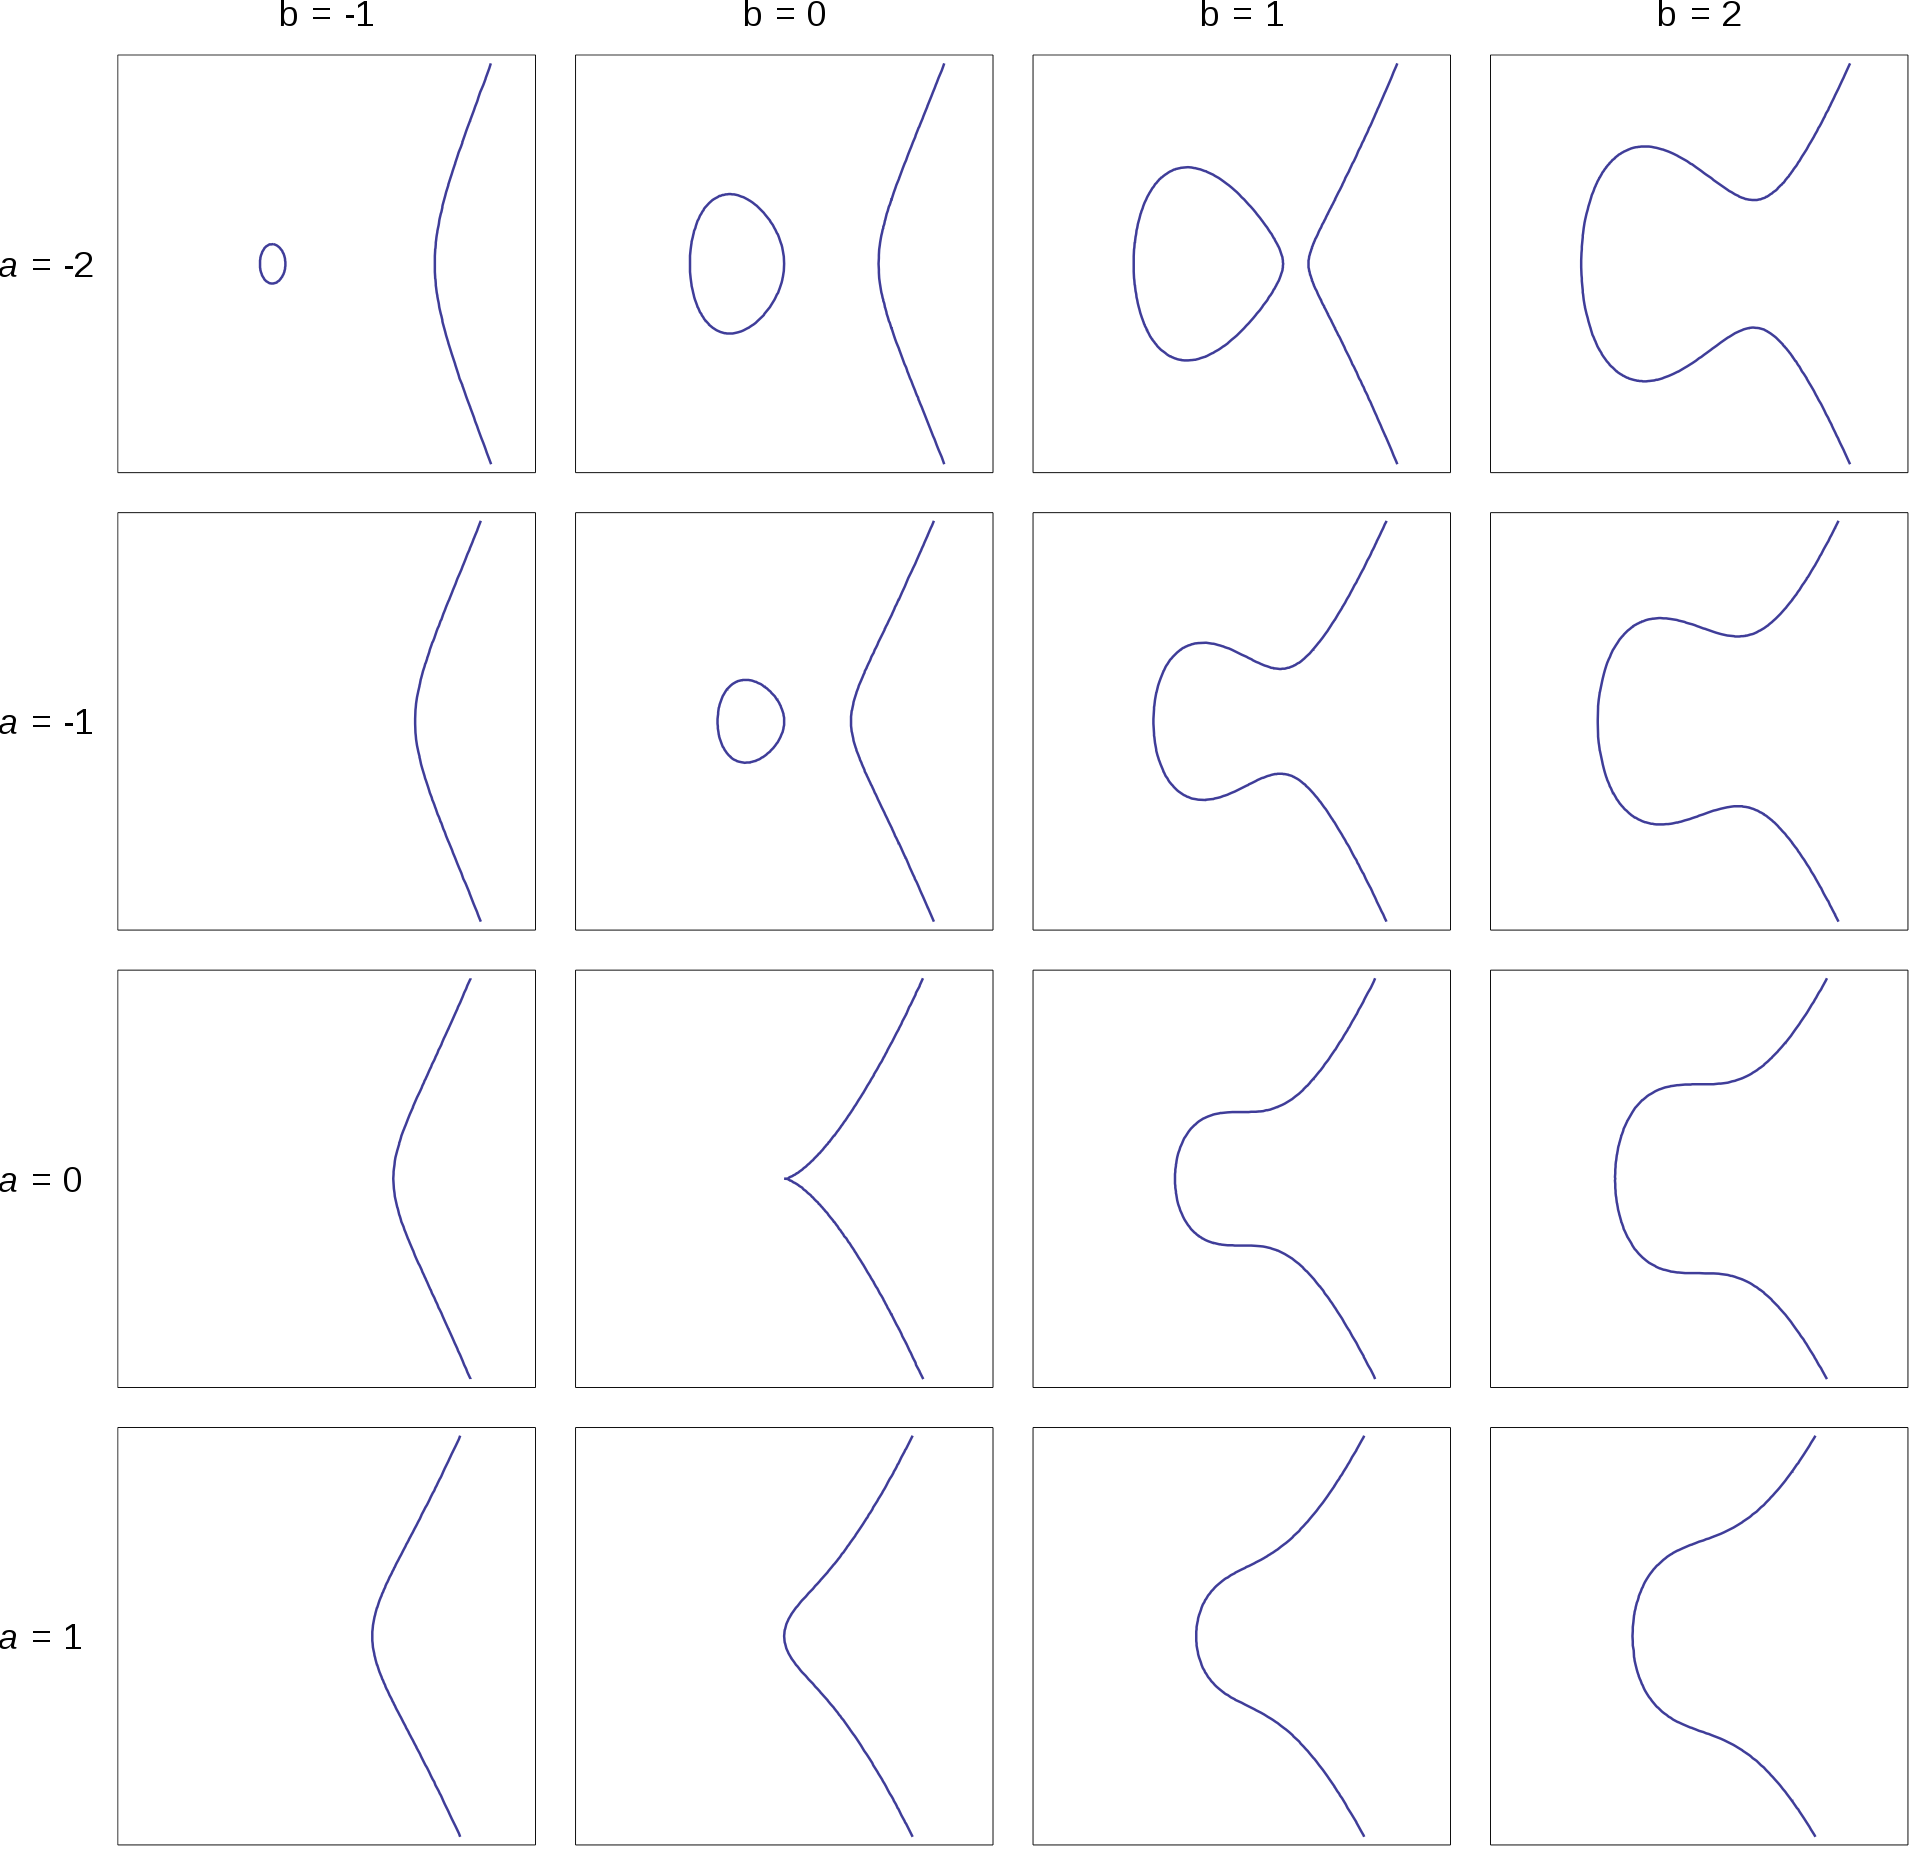
\includegraphics[width=0.55\textwidth]{ec}
  \end{center}
\end{frame}

\begin{frame}
  \frametitle{Elliptic Curves 2/3}
  \begin{itemize}
  \item Elliptic curves are defined over a \textbf{field} $K$ and describes
    points in $K \times K$.
  \item \textbf{Group law}:
    \begin{itemize}
    \item If $P$ and $Q$ are two points on the curve, then we can uniquely
      describe a third point, $P + Q$, in the following way. First, draw the
      line that intersects $P$ and $Q$. This will generally intersect the curve
      at a third point, $R$. We then take $P + Q$ to be $-R$, the point opposite
      $R$.
    \end{itemize}
  \end{itemize}
  \begin{center}
    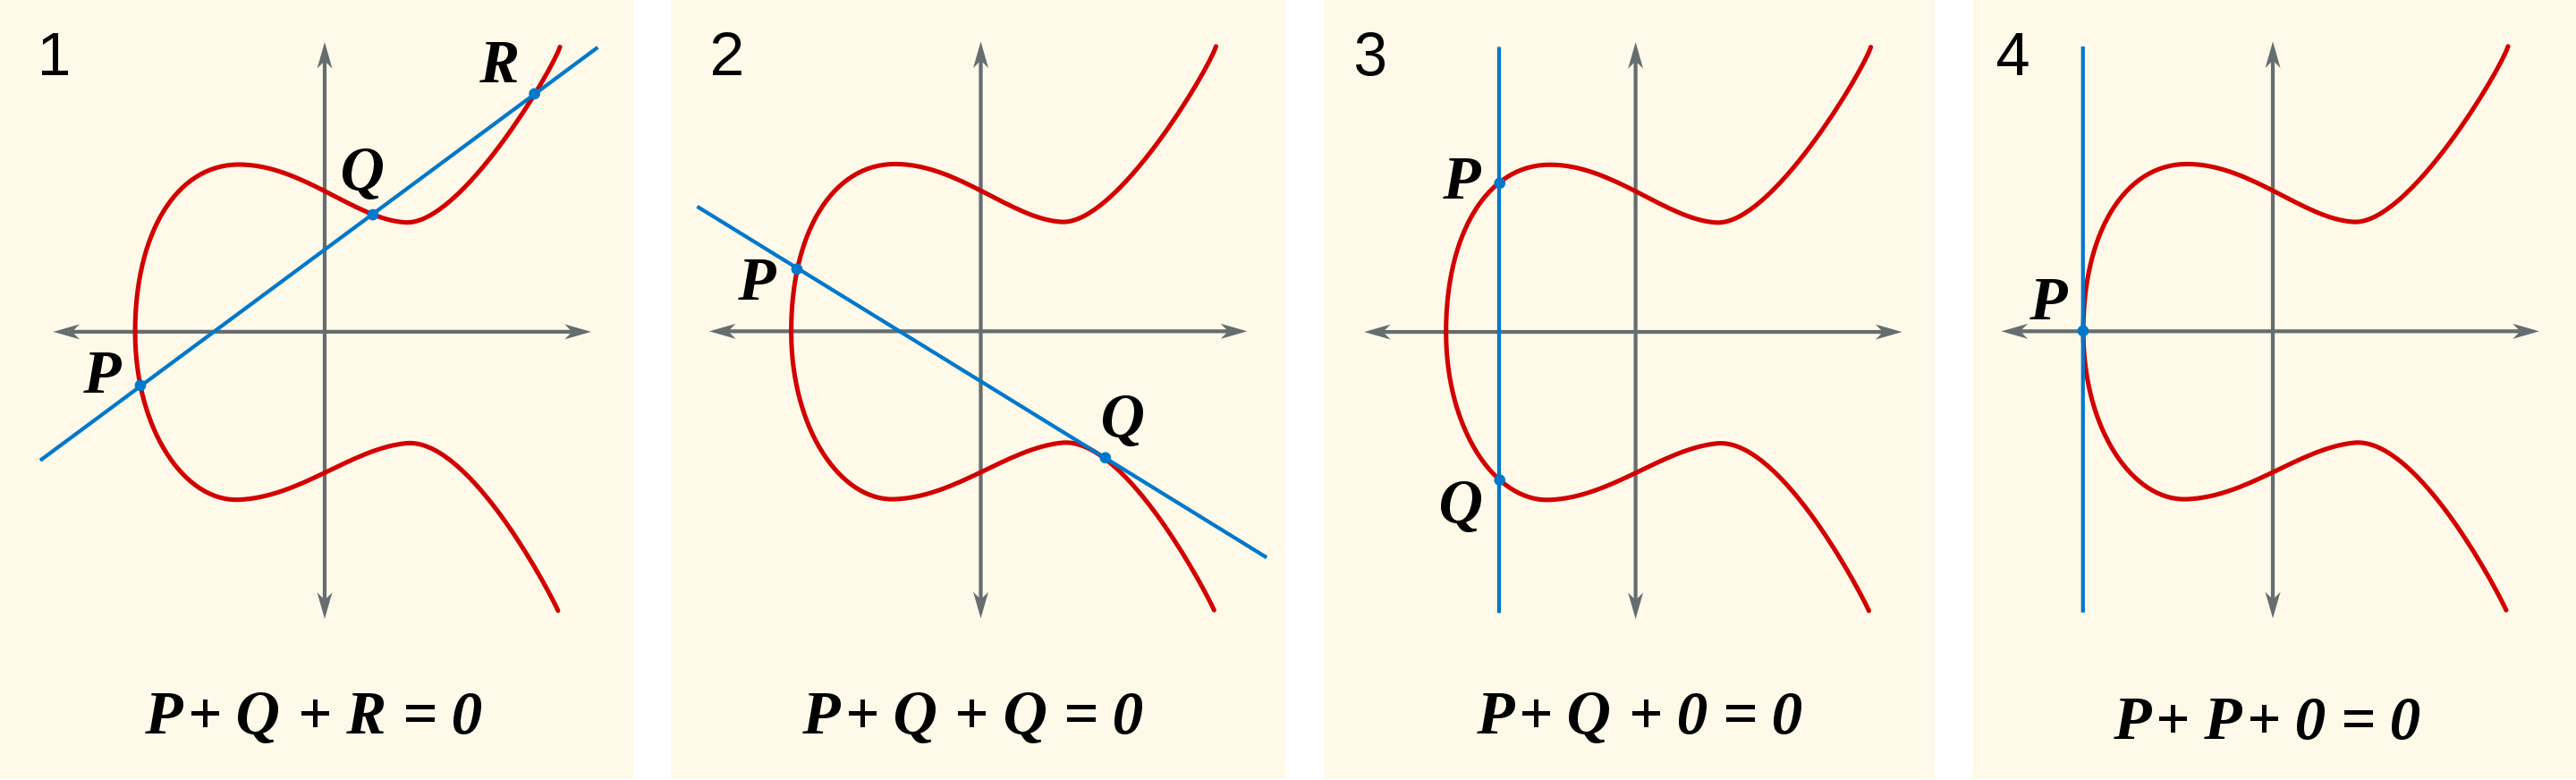
\includegraphics[width=0.9\textwidth]{ec_group}
  \end{center}
\end{frame}

\begin{frame}
  \frametitle{Elliptic Curves 3/3}
  \begin{itemize}
  \item \textbf{Elliptic curves defined over finite fields of prime order} form
    groups that are well suited for cryptographic purposes because of
    significantly \textbf{more complex group structure}, which allows for much
    \textbf{smaller keys}.
  \item An example of an elliptic curve defined over finite filed ($y^2 = x
    ^3 - x$ over $F_{71}$):
  \end{itemize}
  \begin{center}
    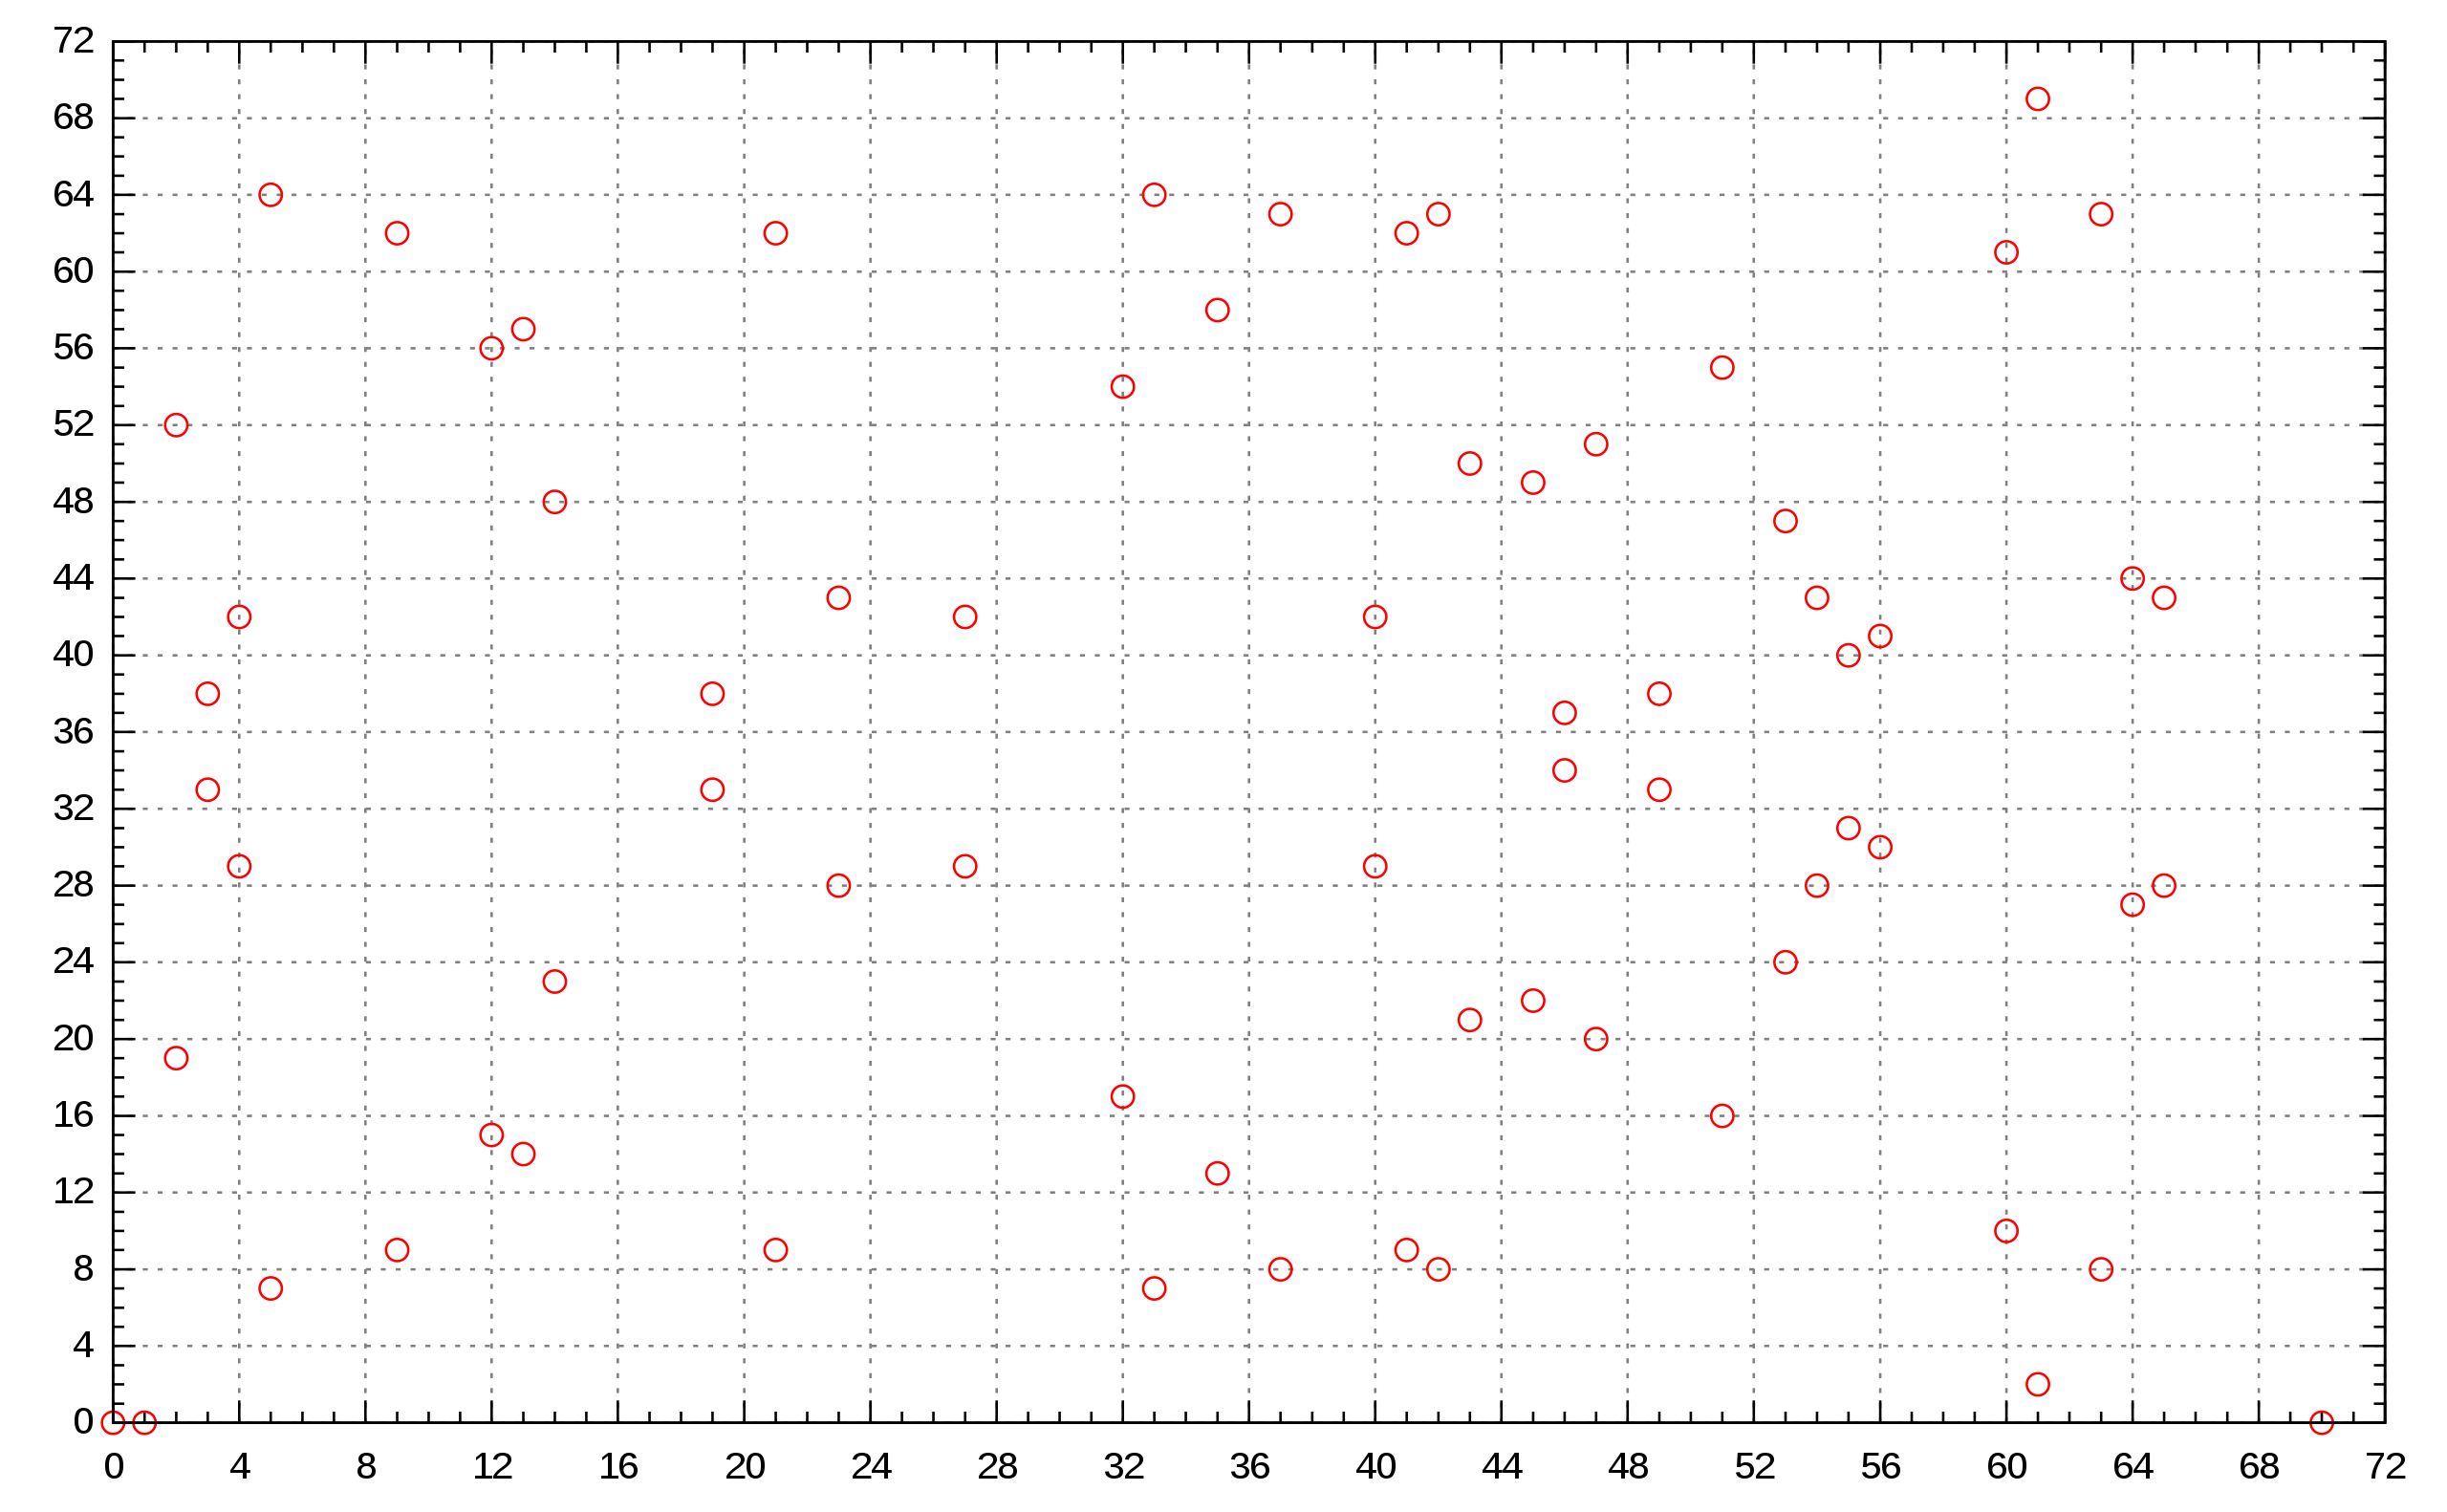
\includegraphics[width=0.7\textwidth]{ec_finite_field_group}
  \end{center}
\end{frame}

\begin{frame}
  \frametitle{Cryptographic Signatures}
  \begin{itemize}
  \item \textbf{Cryptographic signature scheme} is a system for verifying the
    authenticity of messages.
  \item A cryptographic signature scheme consists of the following three
    algorithms:
    \begin{itemize}
    \item a key generation algorithm $Gen$ that selects a private key uniformly
      at random from a set of possible private keys,
    \item a signing algorithm $Sign$ that, given a message and a private key,
      produces a signature,
    \item a signature verification algorithm $Verify$ that, given the message,
      public key and signature, either accepts or rejects the signature.
    \end{itemize}
  \item Successful signature verification provides a \textbf{very strong} reason
    to believe that the particular message was authenticated by the owner of the
    corresponding private key.
  \end{itemize}
\end{frame}

\begin{frame}
  \frametitle{DSA 1/4}
  \begin{itemize}
  \item Alice and Bob must agree on the group parameters $(p, q, Z_p*, G)$, where
    $p$ is prime, $q$ is a smaller prime that divides $p-1$, $Z_p*$ is the multiplicative group of integers modulo $p$,
    $G$ is a generator of a subgroup of $Z_p*$ of order $q$.
  \item Alice creates a key pair, consisting of a private key integer $x$,
    randomly selected from $[1, q - 1]$ and a public key group
    element $y = G^x \pmod{p}$.
  \item To sign a message $m$, Alice
    \begin{itemize}
    \item calculates $e = HASH(m)$,
    \item selects a \textbf{cryptographically secure random integer}
      $k \in [1, q - 1]$ such that $k$ and $q$ are relatively prime,
    \item calculates $r = G^k \pmod{p}$,
    \item calculates $s = k^{-1}(e + x*r) \pmod{q}$.
    \end{itemize}
  \item Signature is a pair $(r, s)$; $(r, -s \pmod{n})$ is \textbf{also valid}.
  \end{itemize}
\end{frame}

\begin{frame}
  \frametitle{DSA 2/4}
  \begin{itemize}
  \item To verify the signature $(r, s)$, Bob
    \begin{itemize}
    \item receives Alice's public key $y$, the message $m$ and the signature $(r, s)$
    \item verifies that $r$ and $s$ are integers in $[1, q - 1]$, otherwise the
      signature is invalid,
    \item calculates $w = s^{-1} \pmod{q}$,
    \item calculates $e = HASH(m)$,
    \item calculates $u_1 = ew$ and $u_2 = rw \pmod{q}$,
    \item calculates the group element $v = G^{u_1} * y^{u_2} \pmod{p} \pmod{q}$.
    \end{itemize}
  \item The signature is valid if $r \equiv v$ and invalid otherwise:
    \begin{align*}
      G^{u_1} * y^{u_2} &= G^{u_1} * G^{u_2x} = G^{u_1 + u_2x} \\
                  &= G^{es^{-1} + rs^{-1}x} = G^{(e + rx)s^{-1}} \\
                  &= G^{(e + rx)(e + rx)^{-1}k} = G^k \\
                  &= r
    \end{align*}
  \end{itemize}
\end{frame}

\begin{frame}
  \frametitle{DSA 3/4}
  \begin{itemize}
  \item To illustrate the process using small numbers:
  \item Global public key elements:
    \begin{itemize}
    \item Choose a prime $p = 23$ and a prime $q = 11$ that divides $p-1$.
    \item Choose an integer $h = 4 (1 < h < p-1)$, then calculate $G = h^{(p-1)/q} \pmod{p} = 4^{(23-1)/11} \pmod{23} = 8$.
    \end{itemize}
  \item Alice's key pair:
    \begin{itemize}
    \item Private key $x$ is a randomly selected integer from $[1, q-1]$, let's say $x = 6$.
    \item Public key $y$ is $G^x \pmod{p} = 8^6 \pmod{23} = 2$.
    \end{itemize}
  \item Message signing:
    \begin{itemize}
    \item Select a random integer $k$ from $[1, q-1]$, let's say $k = 9$.
    \item Computes $r = g^k \pmod{p} \pmod{q} = 8^9 \pmod{23} \pmod{11} = 6 \pmod{11} = 6$.
    \item Say $e = HASH(m) = 8$. Compute $s = k^{-1} * (e + x*r) \pmod{q} = 9^{-1} * (8 + 6*6) \pmod{11} = 5 * (8 + 36) \pmod{11} = 8$.
    \item The signature is $(r, s) = (6, 8)$.
    \end{itemize}
  \end{itemize}
\end{frame}

\begin{frame}
  \frametitle{DSA 4/4}
  \begin{itemize}
  \item Verification (Bob's step):
    \begin{itemize}
    \item Bob receives Alice's public key $y = 2$, the message $m = "Hello"$, and the signature $(r, s) = (6, 8)$.
    \item Bob calculates:
      \begin{itemize}
      \item $w = s^{-1} \pmod{q} = 8^{-1} \pmod{11} = 7$ (because $8*7 \pmod{11} = 1$).
      \item $u_1 = (HASH(m) * w) \pmod{q} = (8 * 7) \pmod{11} = 1$.
      \item $u_2 = (r * w) \pmod{q} = (6 * 7) \pmod{11} = 9$
      \end{itemize}
    \item Finally, Bob checks if $r = (G^{u_1} * y^{u_2} \pmod{p}) \pmod{q} = (8^1 * 2^9 \pmod{23}) \pmod{11} = 6$.
    \end{itemize}
  \item Since r matches, Bob can verify that the signature is from Alice.
  \end{itemize}
\end{frame}

\begin{frame}
  \frametitle{Elliptic Curves 1/3}
  \begin{itemize}
  \item \textbf{Elliptic curves} are algebraic structures described by equations
    of the form:
    $$y^2 = x^3 + ax + b$$
  \end{itemize}
  \begin{center}
    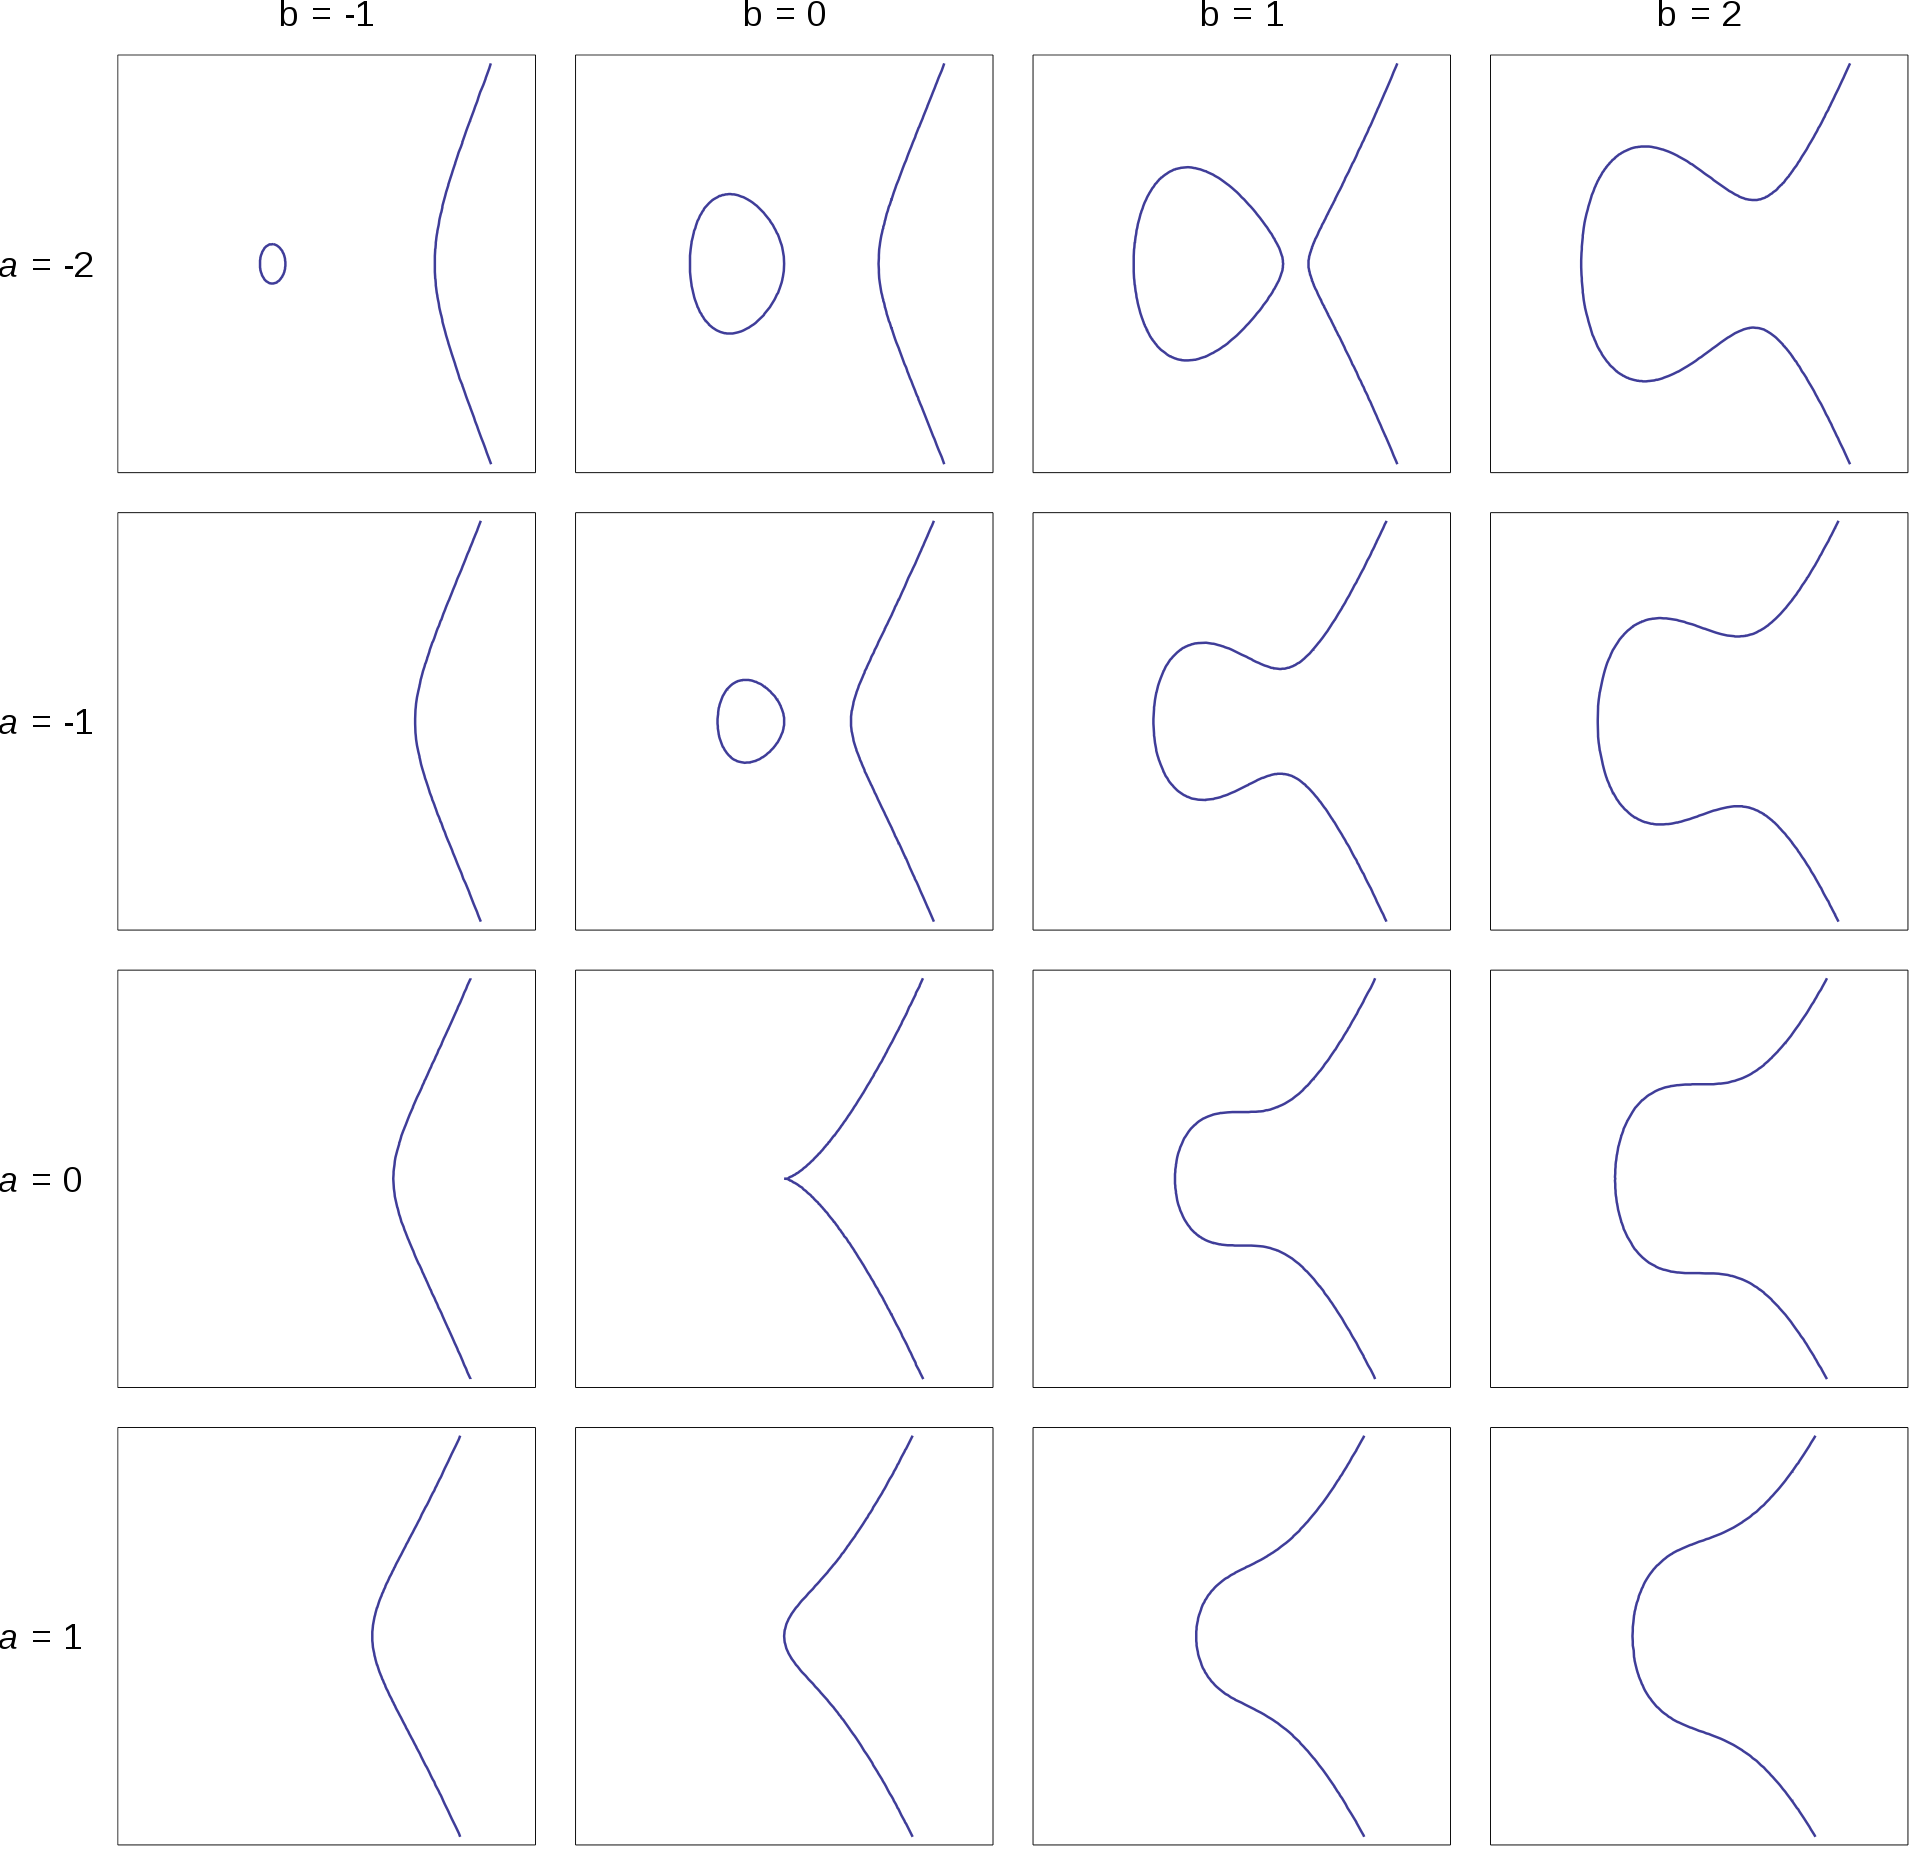
\includegraphics[width=0.55\textwidth]{ec}
  \end{center}
\end{frame}

\begin{frame}
  \frametitle{Elliptic Curves 2/3}
  \begin{itemize}
  \item Elliptic curves are defined over a \textbf{field} $K$ and describes
    points in $K \times K$.
  \item \textbf{Group law}:
    \begin{itemize}
    \item If $P$ and $Q$ are two points on the curve, then we can uniquely
      describe a third point, $P + Q$, in the following way. First, draw the
      line that intersects $P$ and $Q$. This will generally intersect the cubic
      at a third point, $R$. We then take $P + Q$ to be $-R$, the point opposite
      $R$.
    \end{itemize}
  \end{itemize}
  \begin{center}
    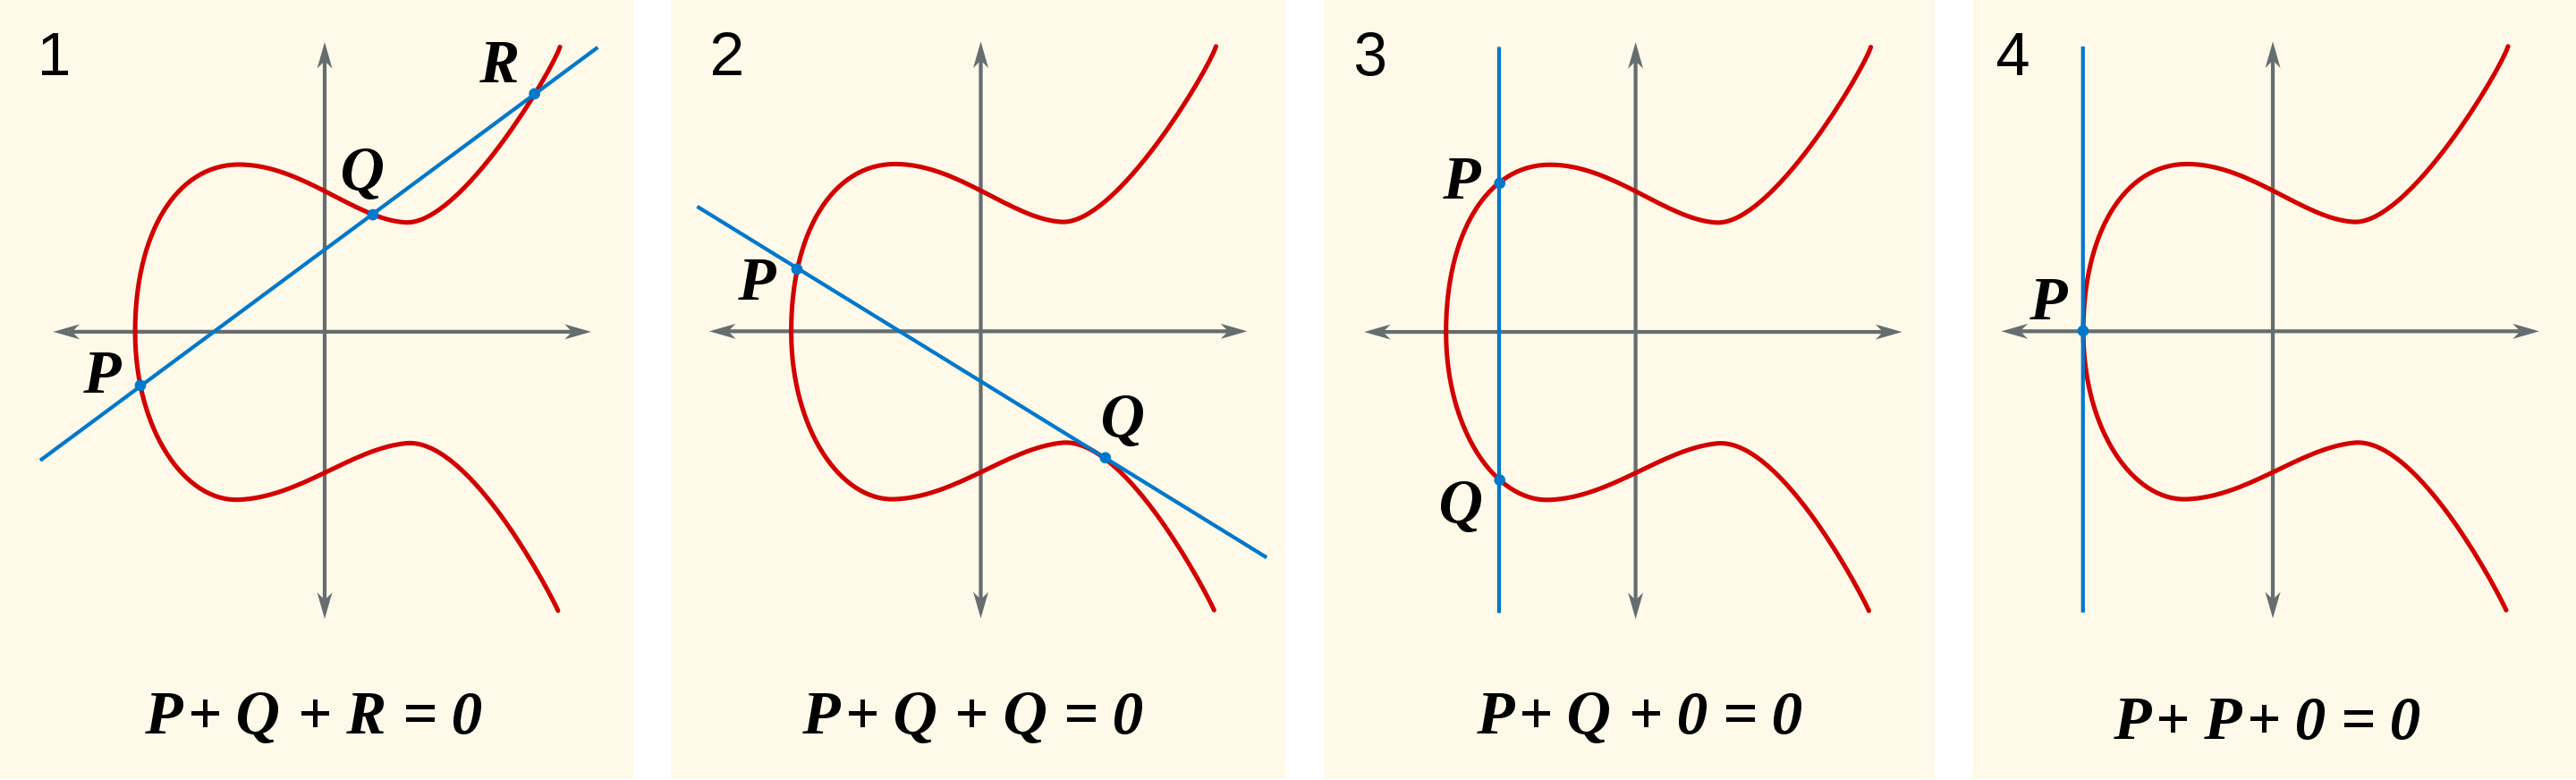
\includegraphics[width=0.9\textwidth]{ec_group}
  \end{center}
\end{frame}

\begin{frame}
  \frametitle{Elliptic Curves 3/3}
  \begin{itemize}
  \item \textbf{Elliptic curves defined over finite fields of prime order} form
    groups that are well suited for cryptographic purposes because of
    significantly \textbf{more complex group structure}, which allows for much
    \textbf{smaller keys}.
  \item An example of an elliptic curve defined over finite field ($y^2 = x
    ^3 - x$ over $F_{71}$):
  \end{itemize}
  \begin{center}
    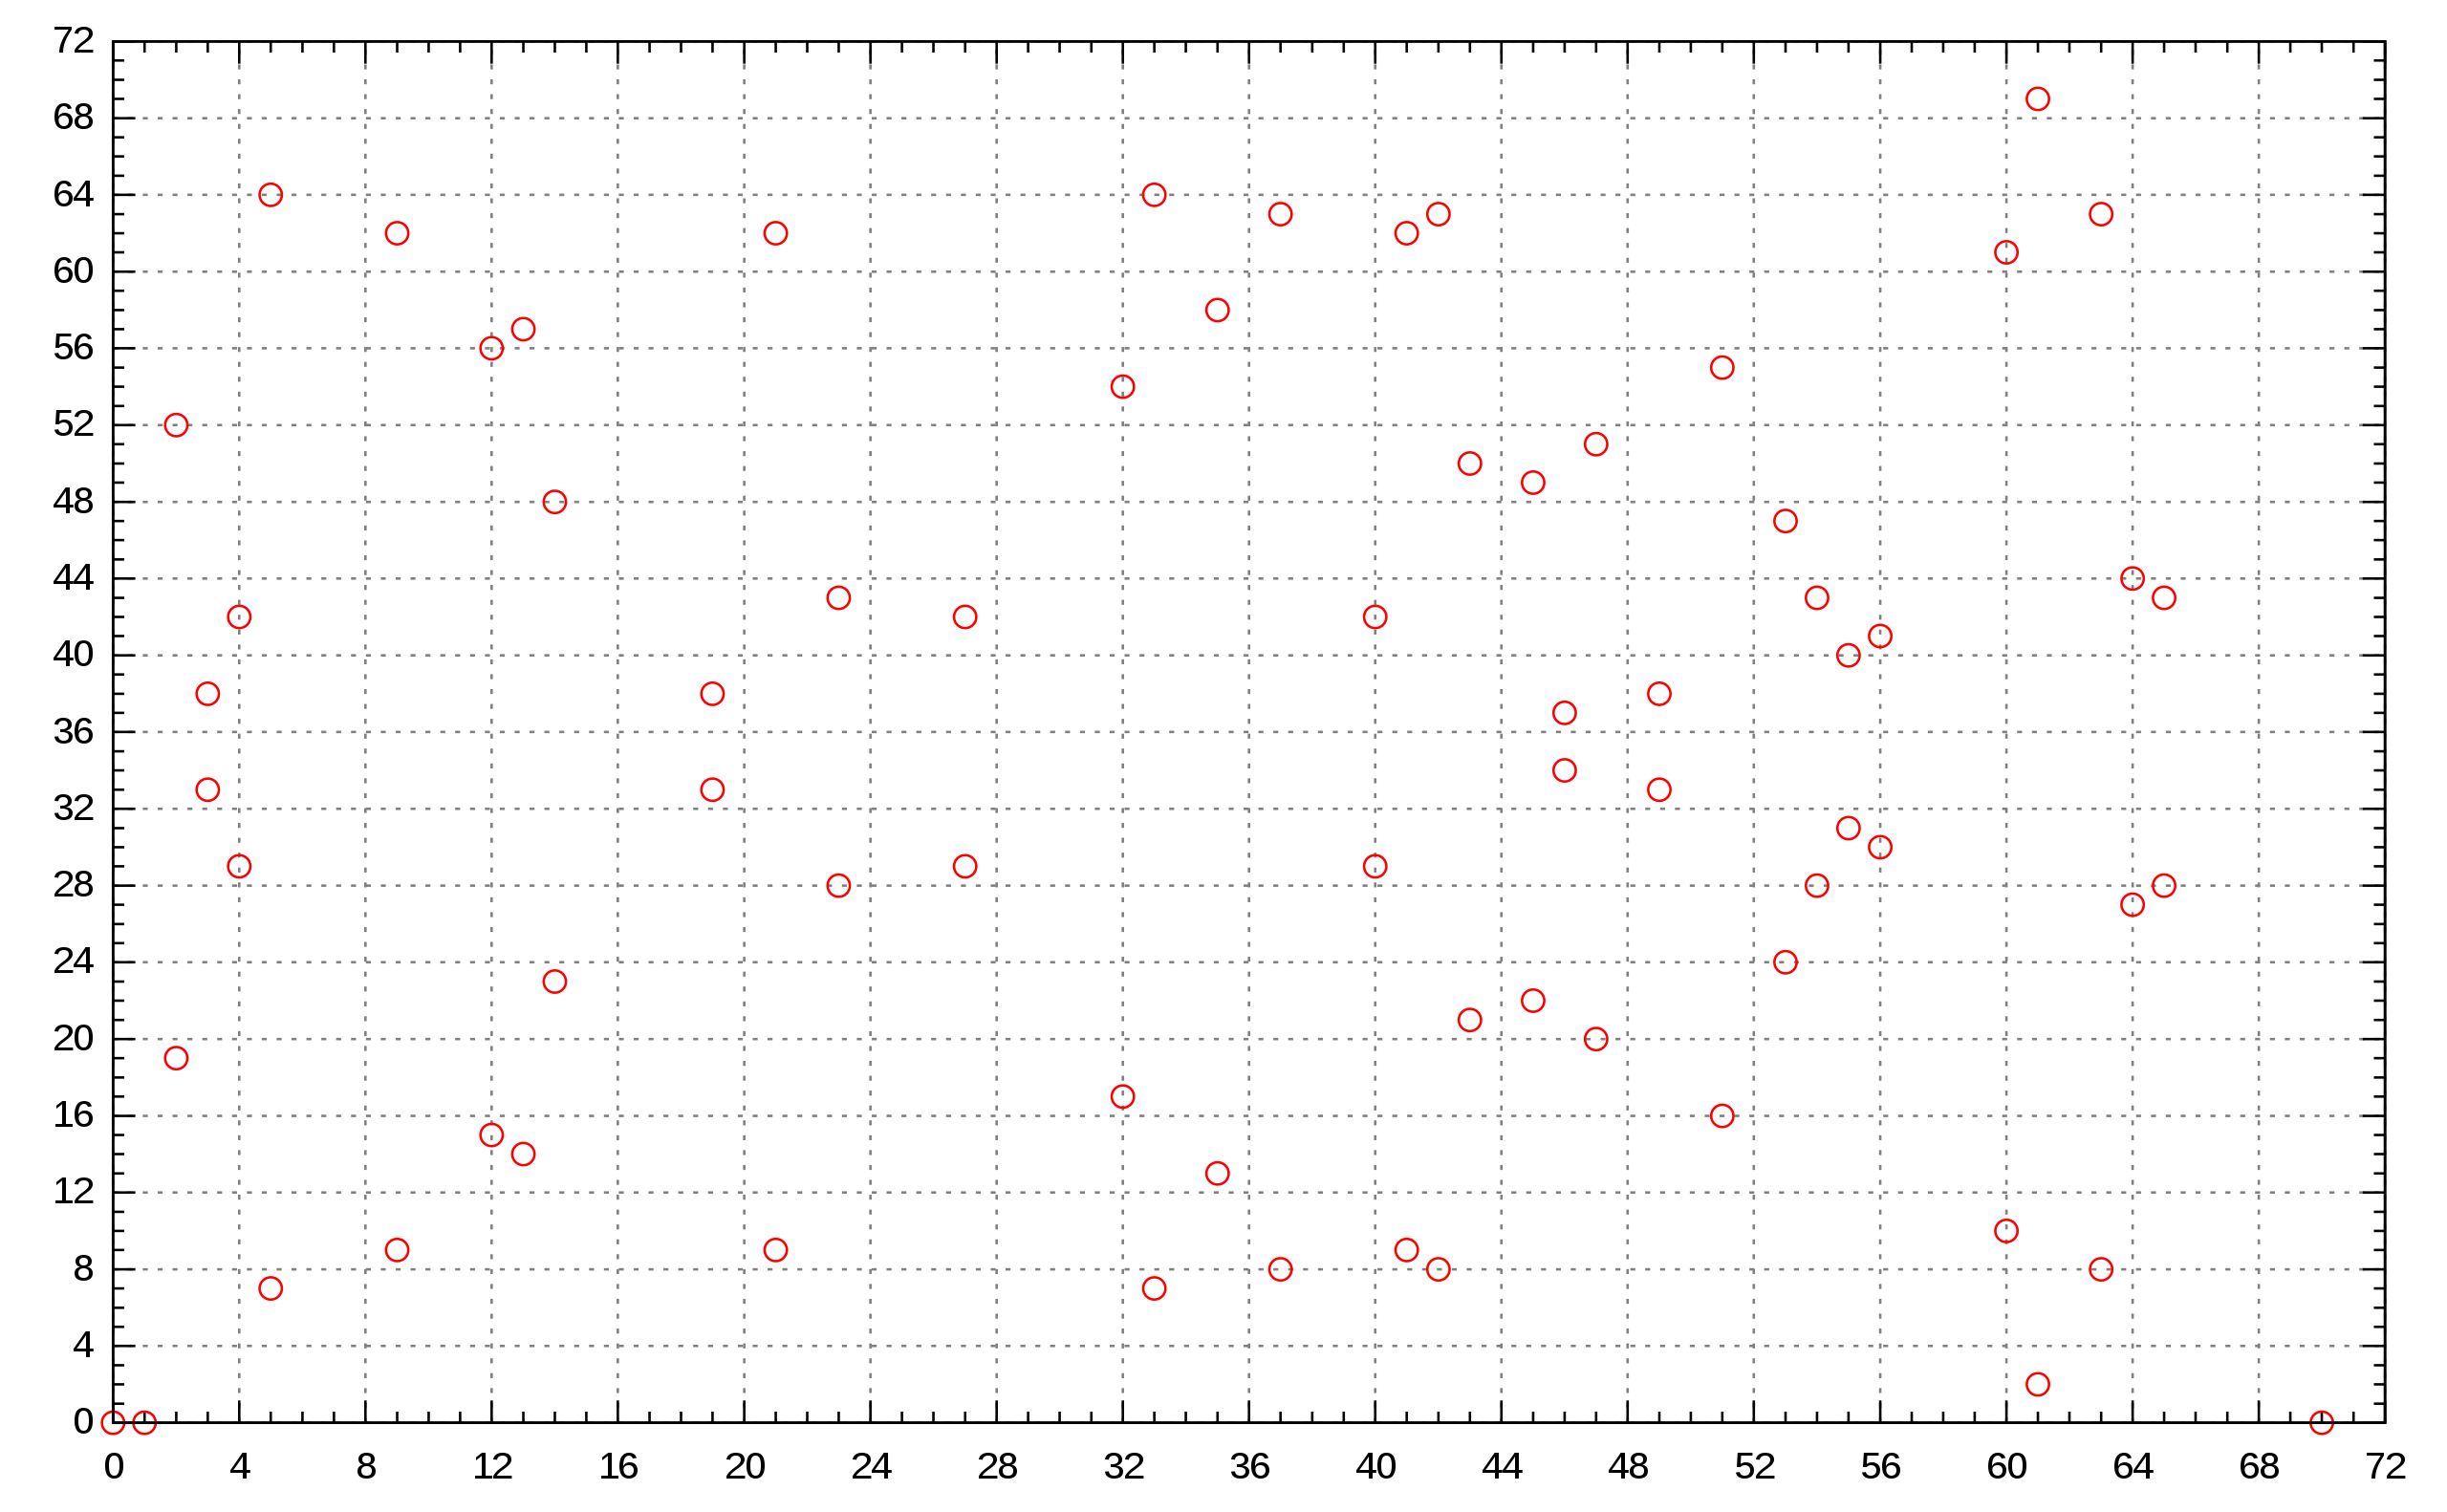
\includegraphics[width=0.7\textwidth]{ec_finite_field_group}
  \end{center}
\end{frame}

\begin{frame}
  \frametitle{ECDSA}
  \begin{itemize}  
  \item \textbf{Elliptic Curve Digital Signature Algorithm} (\textbf{ECDSA}) is
    a variant of the \textbf{Digital Signature Algorithm} (\textbf{DSA}) which
    uses \textbf{elliptic curve cryptography}.
  \item The ECDSA is a variant of the DSA that operates in the group of points on an elliptic curve over a finite field, rather than the multiplicative group of integers modulo a prime.
  \item With \textbf{ECC}, the bit size of the private key believed to be needed
    for ECDSA is about \textbf{twice the size} of the security level, i.e. for
    128 bits of security, the key size of 256 bits is sufficient.
  \item With DSA, the bit size of a key that offers comparable security is 2048
    or even 3072 bits.
  \end{itemize}
\end{frame}

\begin{frame}
  \frametitle{Elliptic Curve SECP256K1 1/2}
  \begin{itemize}
  \item Elliptic curve used in Bitcoin for transaction signing is called
    \textbf{secp256k1}.
    
  \item This elliptic curve is defined over the finite field $F_p$ where
    $$p = 2^{256} - 2^{32} - 2^9 - 2^8 - 2^7 - 2^6 - 2^4 - 1$$
    and is described by the equation
    $$y^2 = x^3 + 7$$
  \end{itemize}
  \begin{center}
    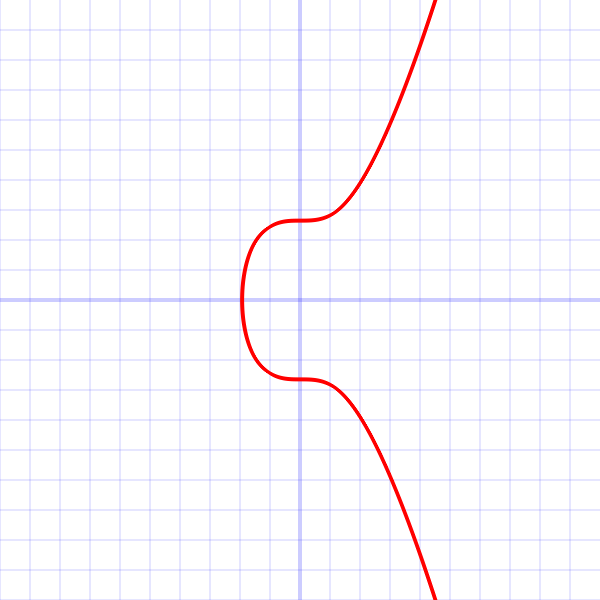
\includegraphics[width=0.3\textwidth]{secp256k1}
  \end{center}
\end{frame}

\begin{frame}
  \frametitle{Elliptic Curve SECP256K1 2/2}
  \begin{itemize}
  \item \textbf{secp256k1} curve is constructed in a special non-random way
    which allows for especially efficient computation.
  \item Unlike other (NIST) elliptic curves used in cryptography (with the
    notable exception of \textbf{curve25519}), \textbf{secp256k1}'s constants
    were selected in a predictable way, which significantly reduces the
    possibility of an existing \textit{backdoor}.
  \item \textbf{libsecp256k1} is a highly-optimized \textbf{secp256k1} curve
    implementation that was extracted from the Bitcoin Core code base into a
    separate project:
    \begin{center}
      https://github.com/bitcoin-core/secp256k1
    \end{center}
  \item Bitcoin uses \textbf{secp256k1} for traditional ECDSA signatures, as
    well as the Schnorr signatures, introduced as part of the \textbf{Taproot}
    upgrade, which was activated on November 14, 2021.
  \end{itemize}    
\end{frame}

\begin{frame}
  \frametitle{Useful Resources}
  \begin{itemize}
  \item \textbf{A Computational Introduction to Number Theory and Algebra} by
    Victor Shoup
    \begin{itemize}
    \item https://shoup.net/ntb/
    \end{itemize}
  \end{itemize}
\end{frame}

\begin{frame}
  \frametitle{The End}
  \begin{center}
    Thank you!
  \end{center}
\end{frame}

\end{document}

%%% Local Variables:
%%% mode: latex
%%% TeX-master: t
%%% End:
